\documentclass[leqno]{beamer}
\usetheme{Madrid}
\usecolortheme{seahorse}

\usepackage[linesnumbered,algoruled,boxed,lined]{algorithm2e}
\usepackage{amsfonts,amsmath,amssymb}
\usepackage{bbm}
\usepackage{booktabs}
\usepackage{caption}
\usepackage{color}
\usepackage{graphicx}
\graphicspath{{./}{../image/}} % graphic path
\usepackage{hyperref}
\hypersetup{colorlinks,citecolor=blue,linkcolor=[RGB]{50,50,172}}
\usepackage{multicol}
\usepackage{multirow}
\usepackage[authoryear]{natbib}
\usepackage{setspace}
\usepackage{soul}
\usepackage{textpos}
\usepackage{tikz}

%% notations; only define those you use frequently
\newcommand{\EE}{{\mathbb{E}}}
\newcommand{\PP}{{\mathbb{P}}}
\newcommand{\QQ}{{\mathbb{Q}}}
\newcommand{\Fb}{\mathbf{F}}
\newcommand{\Ib}{\mathbf{I}}
\newcommand{\hb}{\mathbf{h}}
\newcommand{\xb}{\mathbf{x}}
\newcommand{\one}{\mathbbm{1}}
\newcommand{\Ocal}{\mathcal{O}}

% consistent with R manual
\newcommand\pkg[1]{\texttt{#1}}
\let\proglang=\textsf \let\code=\texttt

\setbeamercovered{transparent}
\setbeamertemplate{caption}[numbered]
\setbeamertemplate{enumerate item}[default]
\setbeamertemplate{itemize item}[circle]
\setbeamertemplate{section in toc}[default]
\setbeamertemplate{subsection in toc}[default]

\AtBeginSection[]{
\begin{frame}<beamer>{Overview}
\tableofcontents[currentsection]
\end{frame}}


\title[\textcolor{black}{UNet-HCRF\_EEG}]{\large
UNet-HCRF Integration for Sequence Labeling on EEG Data}

\author[\scalebox{.85}{Xiaohang Ma, Shiying Xiao, Xiaohui Yin}]
{Xiaohang Ma$^1$, Shiying Xiao$^2$, Xiaohui Yin$^2$}

\institute[\scalebox{.85}{UConn}]
{$^1$Department of Mathematics, University of Connecticut \\
$^2$Department of Statistics, University of Connecticut}

\date[December 9, 2024]{
{\small Storrs, CT} \\
{\small December 9, 2024}}

\begin{document}

\begin{frame}[plain]
\titlepage
\end{frame}


\begin{frame}
\frametitle{Overview}
\tableofcontents
\end{frame}


\section[Introduction]{Introduction}


\begin{frame}{Introduction}
\begin{itemize}
\setlength{\itemsep}{1.5em}
\item Electroencephalography (EEG) pattern recognition tasks are crucial for
healthcare, where accurate and timely data classification can significantly
impact patient outcomes.
\item Deep learning has recently emerged as a powerful tool for sequence
labeling.
\item Conditional random fields (CRFs) have been employed for modeling label
dependencies, demonstrating promising results.
\end{itemize}
\end{frame}


\begin{frame}{Framework}
\begin{figure}[tbp]
\centering
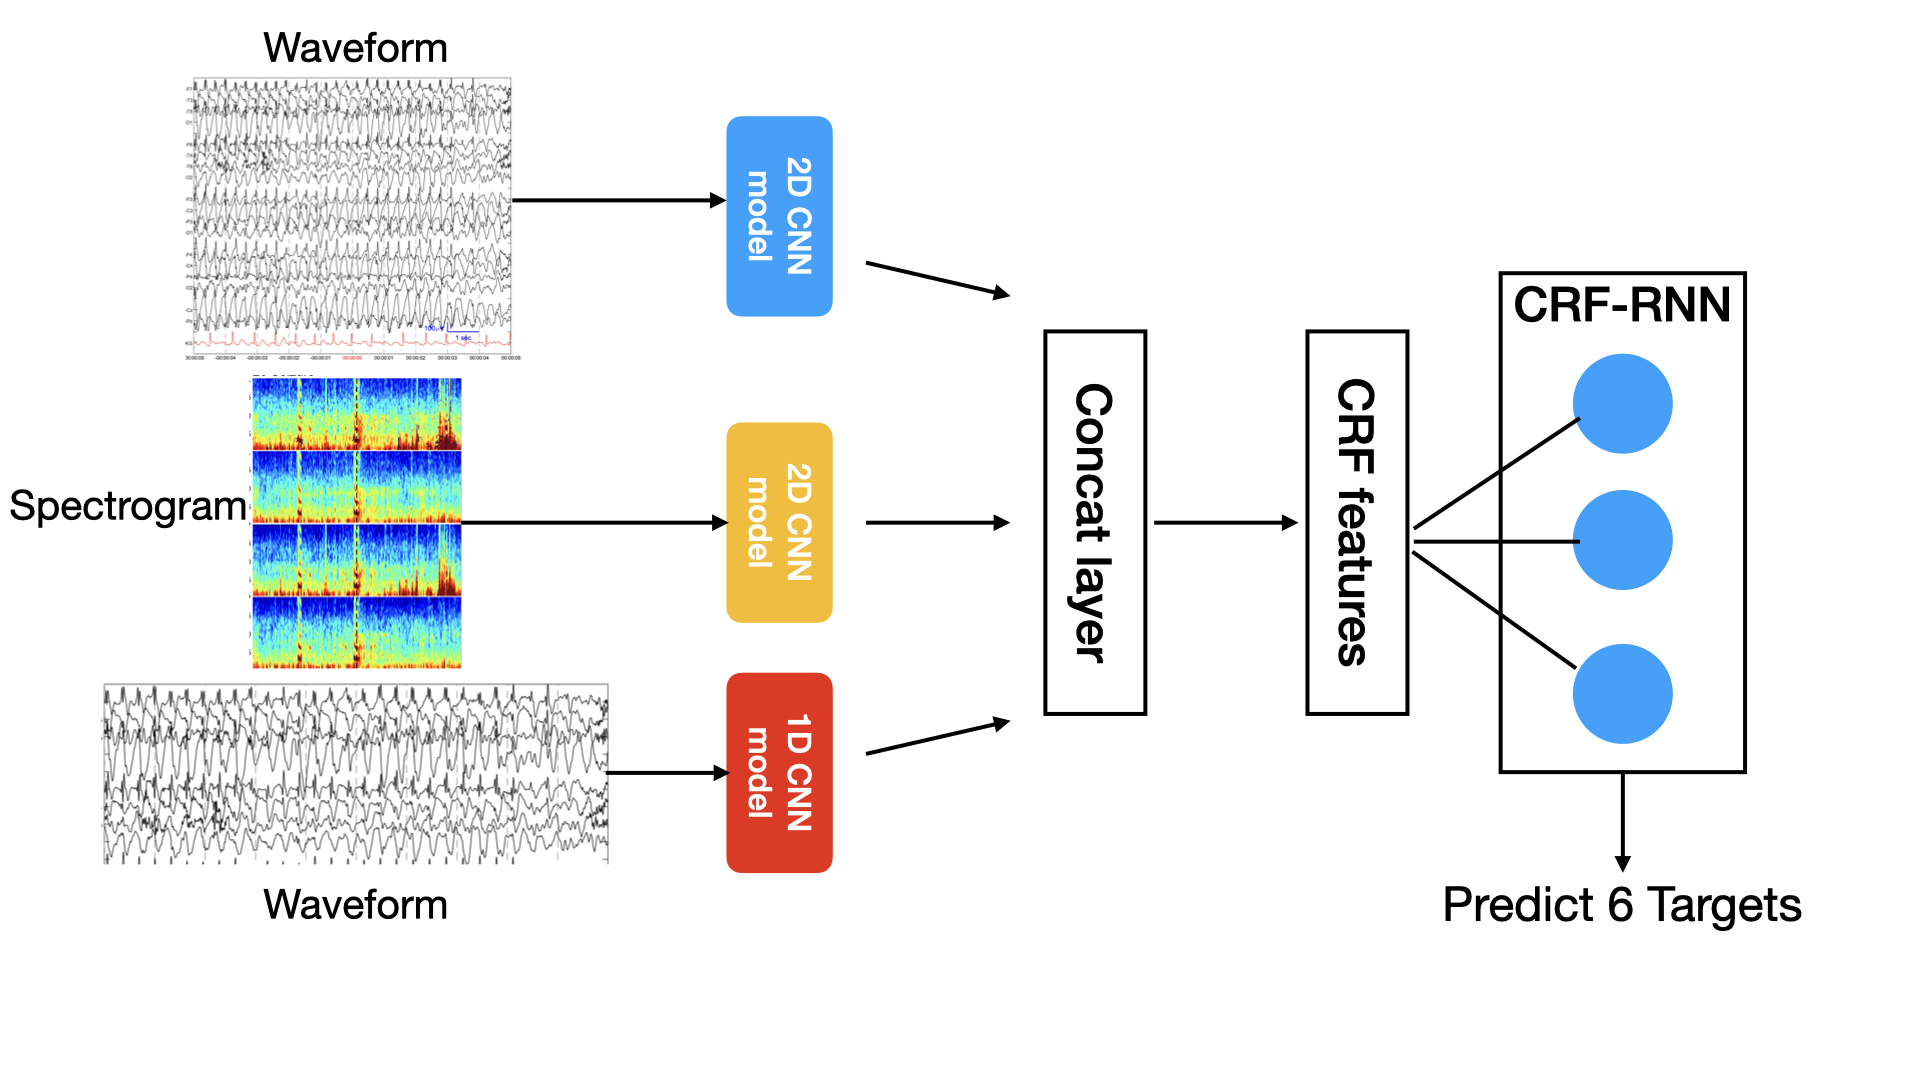
\includegraphics[width=\textwidth]{model}
\end{figure}
\end{frame}


\section[Methods]{Methods}


\begin{frame}{CNN-HCRF Model Structure}
\begin{itemize}
\item Given the feature of the input data $\Ib$ learned by CNN, i.e.
$\xb = \Fb(\Ib)$, its corresponding hidden part states $\hb$, and the class
label $y$, a hidden conditional random field (HCRF) has the exponential form:
\begin{equation*}
\PP(y, \hb \vert \xb; \theta)
= \frac{\exp\left(\Phi(y, \hb, \xb; \theta)\right)}
{\sum_{y^\prime \in Y} \sum_{\hb \in H^N}
\exp\left(\Phi(y^\prime, \hb, \xb; \theta)\right)},
\end{equation*}
where $\theta$ is the model parameter, $H^N$ denotes the set of all possible
hidden part states of $N$ hidden parts, and $\Phi(y, \hb, \xb; \theta)$
refers to potential function depending on the feature $\xb$.
\item The probability of class label $y$ for the given feature $\xb$ is:
\begin{equation*}
\PP(y \vert \xb; \theta) = \sum_{\hb \in H^N} \PP(y, \hb \mid \xb; \theta)
= \frac{\sum_{\hb \in H^N} \exp\left(\Phi(y, \hb, \xb; \theta)\right)}
{\sum_{y^\prime \in Y} \sum_{\hb \in H^N}
\exp\left(\Phi(y^\prime, \hb, \xb; \theta)\right)}.
\end{equation*}
\end{itemize}
\end{frame}


\begin{frame}{CNN-HCRF Model Structure (cont.)}
The jointly probability distribution of the HCRF model is:
\begin{align*}
\Phi(y, \hb, \xb; \theta) &= \underbrace{
\sum_{j \in \nu} \phi(h_j, x_j; \omega) +
\sum_{i \neq j} \psi(h_i, h_j, x_i, x_j; \eta)}_{
% \propto \log\PP( \hb \vert \xb; \theta)
\textrm{Measures log-likelihood $\log\PP(\hb \vert \xb; \theta)$}} \\
& + \underbrace{
\sum_{j \in \nu} \varphi(y, h_j, x_j; \delta) + \vartheta(y, x_0; \varpi)}_{
% \propto \log\PP(y | \hb, \xb; \theta)
\textrm{Measures log-likelihood $\log\PP(y \vert \hb, \xb; \theta)$}},
\end{align*}
where:
\begin{itemize}
\item Unary potential $\phi(h_j, x_j; \omega)$: Measures the likelihood of the
local feature $x_j$ is assigned as the hidden part state $h_j$, with parameter
$\omega$ is learned by end-to-end CNN-UNet structure.
\end{itemize}
\end{frame}


\begin{frame}{CNN-HCRF Model Structure (cont..)}
\begin{itemize}
\item Binary potential $\psi(h_i, h_j, x_i, x_j; \eta)$: Balances the hidden
label compatibility of the neighboring pixels $p$ on the feature $\xb$:
\begin{align*}
\psi(h_i, h_j, x_i, x_j; \eta) &= \mu(h_i, h_j) \Bigg[
\omega_1 \exp \left(
-\frac{\left\lvert p_i - p_j \right\rvert^2}{2\eta_\alpha^2}
-\frac{\left\lvert x_i - x_j \right\rvert^2}{2\eta_\beta^2}
\right) \\
&+ \omega_2 \exp \left(
- \frac{\left\lvert p_i - p_j \right\rvert^2}{2 \eta_\gamma^2}
\right)
\Bigg],
\end{align*}
where $\mu(h_i, h_j)$ is a label compatibility function,
%that describes the interactive influences between different pairs of classes.
$\omega_1$ and $\omega_2$ are linear combination weights of different kernels,
and the parameters $\eta_\alpha$, $\eta_\beta$ and $\eta_\gamma$ control the
influence of the corresponding feature spaces.
\end{itemize}
\end{frame}


\begin{frame}{CNN-HCRF Model Structure (cont...)}
\begin{itemize}
\item Unary potential $\varphi(y, h_{j}; \delta)$: Measures the compatibility
between global class label $y$ and the hidden local state $h_j$:
\begin{equation*}
\varphi(y, h_{j}; \delta) = \sum_{a \in Y} \sum_{b \in H} \delta_{a, b}
\cdot \one(y = a) \cdot \one(h_j = b),
\end{equation*}
where $\one(\cdot)$ is a indicator function, and $\delta_{a,b}$ denotes the
likelihood of class label $y = a$ containing a joint with hidden state
$h_j = b$, learned during training.
\item Global potential $\vartheta(y, x_0; \varpi)$: Measures the likelihood of
the global feature $x_0$ is assigned as the action label $y$, with parameter
$\varpi$ learned during training process.
\end{itemize}
\end{frame}


\begin{frame}{Variational Inference of HCRF}
\begin{small}
\begin{itemize}
\item The mean-field varepsilon family approximation of
$\log P(\hb \mid y,\xb,\theta)$ is expressed as
$\QQ(h) = \prod_{i=1}^N q_i(h_i)$.
\item The evidence lower bound (ELBO) under the mean-field family is:
\begin{equation*}
\begin{split}
& \mathrm{ELBO}(\QQ) = \EE_{\QQ(\hb)} \log\PP(y, \hb \vert \xb; \theta)
- \EE_{\QQ(\hb)} \log q(\hb) \\
&\quad = \sum_{i=1}^N \EE_{q_i(h_i)}
\left[ \phi(h_j, x_j; \omega) + \varphi(y, h_j, x_j; \delta) \right] \\
&\quad + \sum_{i=1}^N \sum_{j=1}^N \sum_{l,l^\prime} \one_{\{i \neq j\}} 
\QQ(h_i = l) \QQ(h_j = l^\prime) \mu(l, l^\prime) \\
&\quad \left[ \omega_1 \exp \left(
- \frac{\left\lvert p_i - p_j \right\rvert^2}{2\eta_\alpha^2}
- \frac{\left\lvert \Fb_i(\Ib) - \Fb_j(\Ib) \right\rvert^2}{2\eta_\beta^2}
\right) + \omega_2 \exp \left(
- \frac{\left\lvert p_i - p_j \right\rvert^2}{2\eta_\gamma^2}
\right) \right] \\
&\quad - \sum_{i=1}^N \EE_{q_i} \log q_i(h_i) + \vartheta(y, \xb; 
\varpi).
\end{split}
\end{equation*}
\end{itemize}
\end{small}
\end{frame}


\begin{frame}{Variational Inference of HCRF (cont.)}
\begin{itemize}
\item By the coordinate ascent variational inference (CAVI) algorithm, fixing
$q_j(h_j), \forall j \neq i$, the optimal $q_i(h_i)$ that maximizes
$\mathrm{ELBO}(q_i(h_i))$ is:
\begin{equation*}
\QQ(h_i) \propto \exp\{\EE_{\QQ(\hb_{-i})}
\log\PP(y, h_i, \hb_{-i} \mid \xb; \theta)\}.
\end{equation*}
\item The explicit form of $q_i(l)$ is derived as follows:
\begin{equation*}
\begin{split}
& q_i(l) = \frac{1}{Z_i} \exp \Bigg\{
\phi(h_j, x_j; \omega) + \varphi(y, h_j, x_j; \delta)
+ \sum_{j \neq i} \sum_{l^\prime} q(l^\prime) \mu(l, l^\prime) \\
& \left[ \omega_1 \exp \left(
- \frac{\left\lvert p_i - p_j \right\rvert^2}{2\eta_\alpha^2}
- \frac{\left\lvert \Fb_i(\Ib) - \Fb_j(\Ib) \right\rvert^2}{2\eta_\beta^2}
\right)
+ \omega_2 \exp \left(
- \frac{\left\lvert p_i - p_j 
\right\rvert^2}{2\eta_\gamma^2}
\right)
\right]
\Bigg\},
\end{split}
\end{equation*}
where $Z_i$ is the normalization constant.
\end{itemize}
\end{frame}


%\begin{frame}{Model Structure}
%\begin{small}
%\begin{itemize}
%\item An Unet CNN was designed to generated a feature map, and a global
%potential for the label.
%\item A hidden CRF layer will address the pixel wise label information of the
%feature map, then assign a latent label $h_i$ at each pixel.
%\item The latent label $h_i$ will contribute the global feature through the
%following potetial.
%\begin{equation*}
%\varphi(y, h_{j}; \delta) = \sum_{a \in Y} \sum_{b \in H} \delta_{a, b}
%\cdot \one(y = a) \cdot \one(h_j = b)
%\end{equation*}
%\item The jointly probability distribution of the model
%\begin{equation*}
%\begin{split}
%\Phi(y, \hb, \xb; \theta) &= \underbrace{
%\sum_{j \in \nu} \phi(h_j, x_j; \omega)
%+ \sum_{i \neq j} \psi(h_i, h_j, x_i, x_j; \eta)}_{
%% \propto \log\PP(\hb \vert \xb; \theta)
%\textrm{Measures log-likelihood $\log\PP(\hb \vert \xb; \theta)$}} \\
%&+ \underbrace{
%\sum_{j \in \nu} \varphi(y, h_j, x_j; \delta) + \vartheta(y, \xb; \varpi)}_{
%% \propto \log\PP(y | \hb,  \xb; \theta)
%\textrm{Measures log-likelihood $\log\PP(y \vert \hb, \xb; \theta)$}}
%\end{split}
%\end{equation*}
%\end{itemize}
%\end{small}
%\end{frame}


%\begin{frame}{Model Inference}
%\begin{small}
%\begin{itemize}
%\item The inference for the latent variable follows a standard mean-field
%Variational Inference scheme.
%\begin{equation*}
%\QQ(h_i) \propto \exp\{\EE_{\QQ(\hb_{-i})}
%\log\PP(y, h_i, \hb_{-i} \vert \xb; \theta)\}.
%\end{equation*}
%\item The resulting ELBO will be used as predicted log-likelihood of each 
%image:
%\begin{equation*}
%\begin{split}
%& \textrm{ELBO}(\QQ) = \EE_{\QQ(\hb)} \log\PP(y, \hb \vert \xb; \theta)
%- \EE_{\QQ(\hb)} \log q(\hb) \\
%&\quad = \sum_{i=1}^N \EE_{q_i(h_i)}
%\left[ \phi(h_j, x_j; \omega) + \varphi(y, h_j, x_j; \delta) \right] \\
%&\quad + \sum_{i=1}^N \sum_{j=1}^N \sum_{l,l^\prime} \one_{\{i \neq j\}} 
%\QQ(h_i = l) \QQ(h_j = l^\prime) \mu(l, l^\prime) \\
%&\quad \left[ \omega_1 \exp \left(
%- \frac{\left\lvert p_i - p_j \right\rvert^2}{2\eta_\alpha^2}
%- \frac{\left\lvert \Fb_i(\Ib) - \Fb_j(\Ib) \right\rvert^2}{2\eta_\beta^2}
%\right) + \omega_2 \exp \left(
%- \frac{\left\lvert p_i - p_j \right\rvert^2}{2\eta_\gamma^2}
%\right) \right] \\
%&\quad - \sum_{i=1}^N \EE_{q_i} \log q_i(h_i) + \vartheta(y, \xb; 
%\varpi).
%\end{split}
%\end{equation*}
%\end{itemize}
%\end{small}
%\end{frame}


\section[Experiment]{Experiment}


\begin{frame}{Harmful Brain Activity Classification Dataset}
\begin{itemize}
\item The dataset contains 50-second long EEG samples covering a 10-minute
window as well as spectrograms matching each sample.
\bigskip
\item The EEG samples were labeled by expert annotators to determine which of
the six features each spectrogram belonged to.
\bigskip
\item The longer 10-minute window allows for the model to pick up on further
insights regarding the nature of the brain activity.
\end{itemize}
\end{frame}


\begin{frame}{Data Preparation}
\begin{itemize}
\item Extract 10-minute long spectrograms centered at the midpoint time,
where the expert ratings (Global EEGs) were provided.
\bigskip
\item Convert the 50-second long EEG waveforms into spectrograms.
\end{itemize}
\end{frame}


\begin{frame}{Make Spectrogram from EEG}
\begin{itemize}
\item Bipolar Montage combines multiple EEG electrode signals by calculating
the difference between adjacent electrodes, yielding signals representing
specific brain regions.
\end{itemize}
\begin{figure}[tbp]
\centering
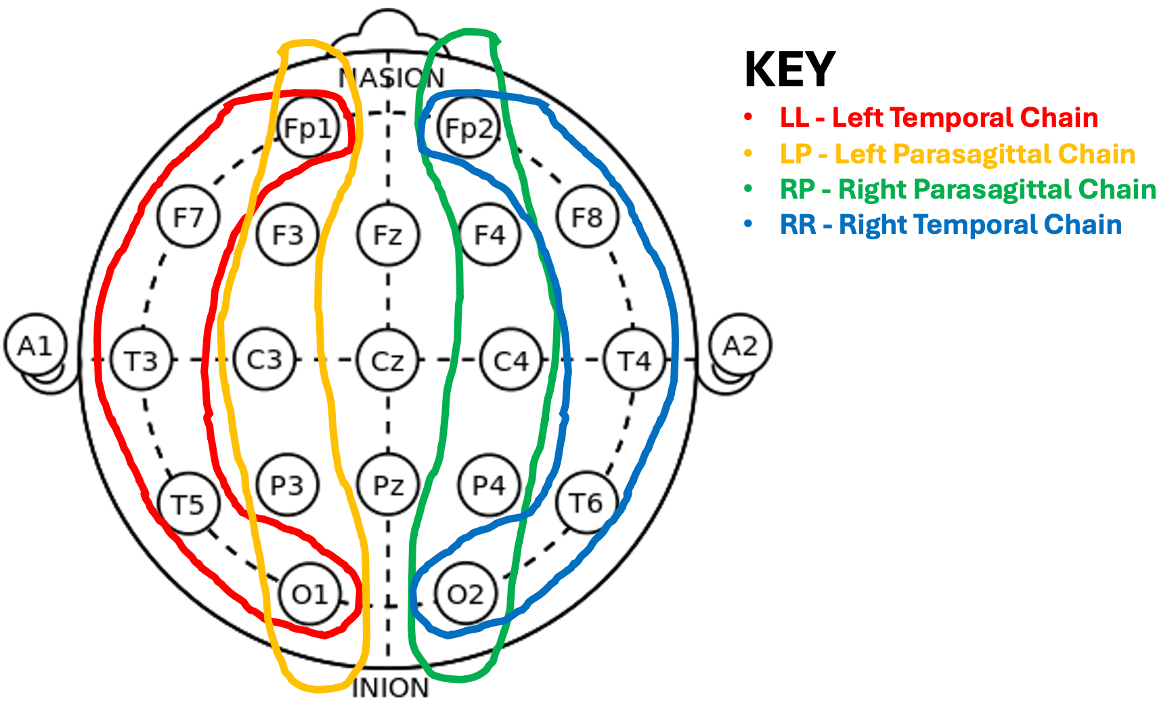
\includegraphics[width=.7\textwidth]{inion}
\end{figure}
\end{frame}


\begin{frame}{Make Spectrogram from EEG (cont.)}
\begin{itemize} 
\item A single time series signal is required to generate a spectrogram.
To create four spectrograms from the dataset's 19 EEG time series signals,
we employ Bipolar Montage to combine them into four representative signals.
\end{itemize}
\begin{footnotesize}
\begin{align*}
& \text{LL Spec} = \frac{1}{4} \left[
spec(Fp1-F7) + spec(F7-T3) + spec(T3-T5) + spec(T5-O1) \right], \\
& \text{LP Spec} = \frac{1}{4} \left[
spec(Fp1-F3) + spec(F3-C3) + spec(C3-P3) + spec(P3-O1) \right], \\
& \text{RP Spec} = \frac{1}{4} \left[
spec(Fp2-F4) + spec(F4-C4) + spec(C4-P4) + spec(P4-O2) \right], \\
& \text{RR Spec} = \frac{1}{4} \left[
spec(Fp2-F8) + spec(F8-T4) + spec(T4-T6) + spec(T6-O2) \right],
\end{align*}
\end{footnotesize}
where $spec(\cdot)$ is a custom function implemented using the \pkg{pywt} and
\pkg{librosa} packages for signal transformation.
\end{frame}


%\begin{frame}{EEG Signal Denosing using Wavelet Transform}
%\begin{enumerate}
%\item Calculates the mean absolute deviation of a signal $d$:
%\begin{equation*}
%\mathrm{maddest}(d, axis) = \frac{1}{N} \sum_{i=1}^N
%\left\vert d_i - \frac{1}{N} \sum_{j=1}^N d_j \right\vert,
%\end{equation*}
%where $d_i$ is the value of the signal at index $i$, and
%$N$ is the length of $d$.
%\item Denoises a signal using wavelet decomposition:
%\begin{enumerate}
%\item Perform wavelet decomposition
%\item Calculate the noise standard deviation using the last level of
%coefficients
%\item Compute the universal threshold
%\item Apply a hard thresholding operation to the coefficients
%\item Reconstruct the signal using the inverse wavelet transform
%\end{enumerate}
%\end{enumerate}
%\end{frame}


\begin{frame}{Make Spectrogram from EEG (cont..)}
\begin{figure}[tbp]
\centering
\vspace{-.5em}
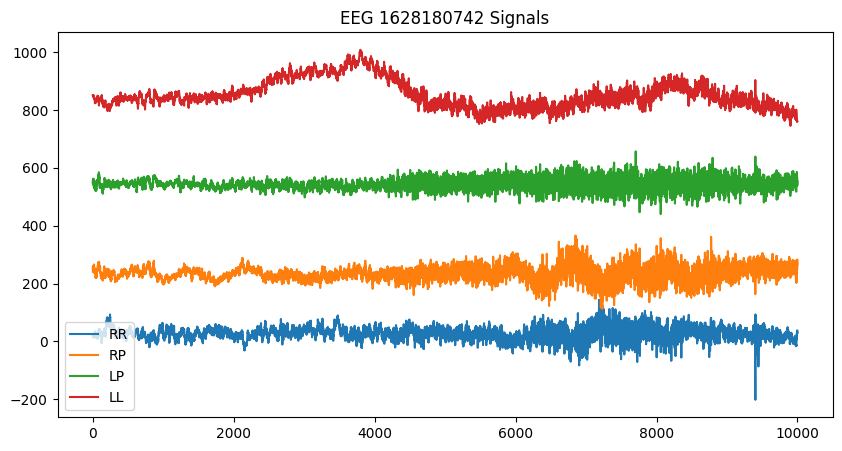
\includegraphics[width=.5\textwidth]{EEG_Signal}
\end{figure}
\vspace{-1em}
\begin{figure}[tbp]
\centering
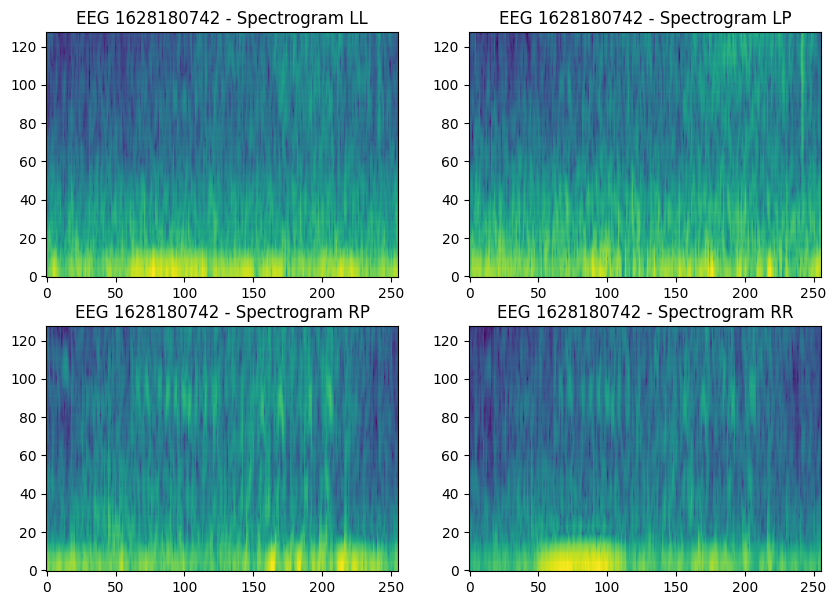
\includegraphics[width=.55\textwidth]{EEG_Spectrogram}
\end{figure}
\end{frame}















%\begin{frame}[allowframebreaks]
%\frametitle{References}
%\bibliographystyle{plain}
%\bibliography{bib}
%\end{frame}

\end{document}
%%% Local Variables:
%%% mode: latex
%%% TeX-master: t
%%% End:
